\documentclass[a4paper]{article}
\usepackage{cmap}  
\usepackage{vntex}
%\usepackage[english,vietnam]{babel}
%\usepackage[utf8]{inputenc}
%\usepackage[utf8]{inputenc}
%\usepackage[francais]{babel}
\usepackage{a4wide,amssymb,epsfig,latexsym,multicol,array,hhline,fancyhdr}

\usepackage{amsmath}
\usepackage{lastpage}
%\usepackage[lined,boxed,commentsnumbered]{algorithm2e}
\usepackage{enumerate}
\usepackage{color}
\usepackage{graphicx}							% Standard graphics package
\usepackage{array}
\usepackage{tabularx, caption}
\usepackage{multirow}
\usepackage{multicol}
\usepackage{rotating}
\usepackage{graphics}
\usepackage{geometry}
\usepackage{float}
\usepackage{setspace}
\usepackage{epsfig}
\usepackage{tikz}
\usetikzlibrary{arrows,snakes,backgrounds}
\usepackage[unicode]{hyperref}
\hypersetup{urlcolor=blue,linkcolor=black,citecolor=black,colorlinks=true} 
%\usepackage{pstcol} 								% PSTricks with the standard color package


\usepackage{pifont}% http://ctan.org/pkg/pifont
\newcommand{\cmark}{\ding{51}}%
\newcommand{\xmark}{\ding{55}}%

%\usepackage{fancyhdr}
\setlength{\headheight}{40pt}
\pagestyle{fancy}
\fancyhead{} % clear all header fields
\fancyhead[L]{
 \begin{tabular}{rl}
    \begin{picture}(25,15)(0,0)
    \put(0,-8){
\includegraphics[width=8mm, height=8mm]{LogoBK.jpg}}
    %\put(0,-8){\epsfig{width=10mm,figure=hcmut.eps}}
   \end{picture}&
	\begin{tabular}{l}
		\textbf{\bf \ttfamily Faculty of Computer Science and Engineering}\\
		\textbf{\bf \ttfamily Bach Khoa University}
	\end{tabular} 	
 \end{tabular}
}
\fancyhead[R]{
	\begin{tabular}{l}
		\tiny \bf \\
		\tiny \bf 
	\end{tabular}  }
\fancyfoot{} % clear all footer fields
\fancyfoot[L]{\scriptsize \ttfamily Đề Tài Xử Lý Ảnh và Thị Giác Máy Tính - Year 2018-2019}
\fancyfoot[R]{\scriptsize \ttfamily Page {\thepage}/\pageref{LastPage}}
\renewcommand{\headrulewidth}{0.3pt}
\renewcommand{\footrulewidth}{0.3pt}


%%%
%\setcounter{secnumdepth}{4}
%\setcounter{tocdepth}{3}
%\makeatletter
%\newcounter {subsubsubsection}[subsubsection]
%\renewcommand\thesubsubsubsection{\thesubsubsection .\@alph\c@subsubsubsection}
%\newcommand\subsubsubsection{\@startsection{subsubsubsection}{4}{\z@}%
%                                     {-3.25ex\@plus -1ex \@minus -.2ex}%
%                                     {1.5ex \@plus .2ex}%
%                                     {\normalfont\normalsize\bfseries}}
%\newcommand*\l@subsubsubsection{\@dottedtocline{3}{10.0em}{4.1em}}
%\newcommand*{\subsubsubsectionmark}[1]{}
%\makeatother



\begin{document}

\begin{titlepage}
\begin{center}
Faculty of Computer Science and Engineering\\
Ho Chi Minh City University of Technology
\end{center}

\vspace{.51cm}

\begin{figure}[h!]
\begin{center}

\includegraphics[width=3cm]{LogoBK.jpg}
\end{center}
\end{figure}

\vspace{0.5cm}


\begin{center}
\begin{tabular}{c}
\multicolumn{1}{l}{\textbf{{\Large \textcolor{blue}{Xử Lý Ảnh Và Thị Giác Máy Tính}}}}\\
~~\\
\hline
\\
\multicolumn{1}{l}{\textbf{{\Large \textcolor{blue}{Đề Tài}}}}\\
\\
\textbf{{\Huge \textcolor{blue}{Nhận Diện Con Người RealTime}}}\\
\\
\hline
\end{tabular}
\end{center}

\vspace{3cm}

\begin{table}[h]
\begin{tabular}{rrll}
\hspace{5 cm} & GV Hướng Dẫn: & Trần Tuấn Anh &\\
& Author: & Nguyễn Thành Đạt & 1510700 \\
& & Huỳnh Nguyễn Trường Thịnh & 1613343 \\ 
& & Huỳnh Thanh Duy& 1510450\\ 
\end{tabular}
\end{table}

\begin{center}
{\footnotesize Bach Khoa, 9/2018}
\end{center}
\end{titlepage}


%\thispagestyle{empty}
\newpage
\tableofcontents
\newpage

%%%%%%%%%%%%%%%%%%%%%%%%%%%%%%%%%
\section{Mô tả đề tài}
\hspace{6mm} Nhận diện danh tính con người qua camera dựa vào đặc điểm trên khuôn mặt. Sử dụng ngôn ngữ Matlab để lập trình và tính toán 

\begin{itemize}
    \item \textbf{Input}: một hình ảnh (hoặc video), hoặc ghi hình trực tiếp qua camera
    \item \textbf{Output}: Khoanh vùng khuôn mặt của từng người trong khung hình và cho biết khuôn mặt đó của người nào
\end{itemize}

\section{Các Bước Thực Hiện}
\subsection{Thu thập dữ liệu}
\begin{itemize}
    \item Dữ liệu được gồm 1000 khuôn mặt của những người bất kỳ được dán nhãn là "Unknown"
    \item Dữ liệu của khuôn mặt người được scan trực tiếp qua camera (ít nhất1200 ảnh / 1 người) 
    \item Sau khi thu thập toàn bộ dữ liệu khuôn mặt người, chuyển đổi hình màu sang hình xám và scale về cùng kích thước là 144x144
\end{itemize}
\begin{figure} [H]
\centering
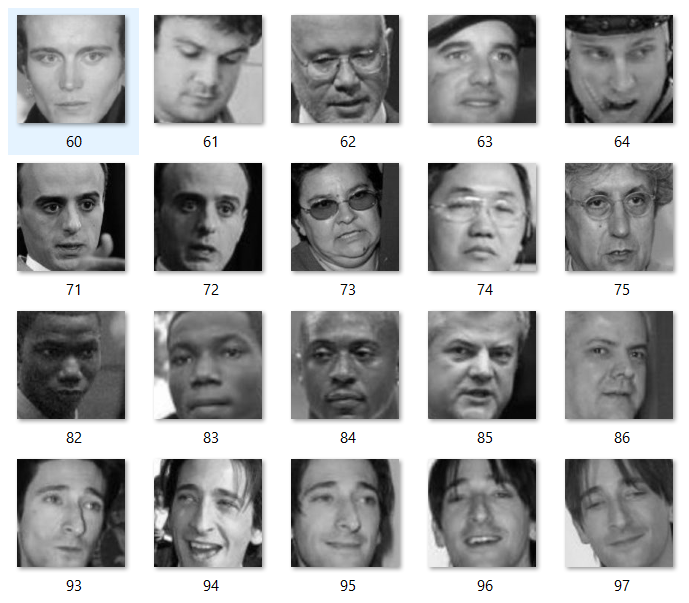
\includegraphics[scale=0.45]{unknown.png}
\caption{Khuôn mặt của bất kỳ người nào, có nhãn "Unknown"}
\label{fig:ts}
\end{figure}

\begin{figure} [H]
\centering
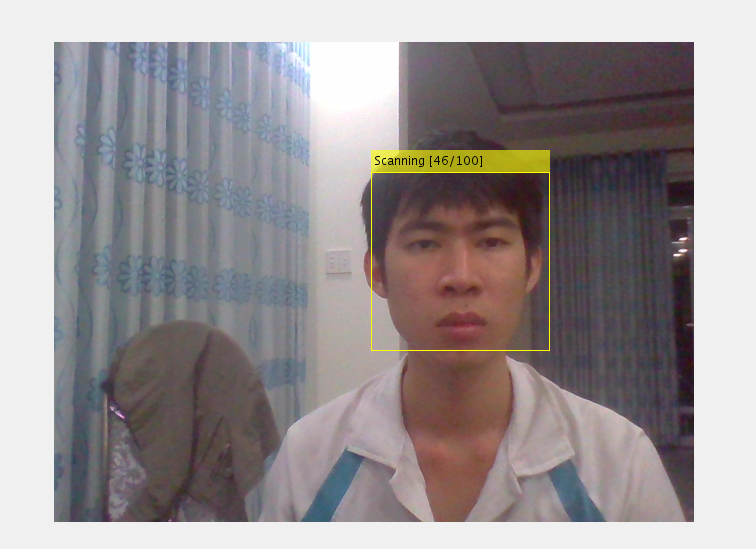
\includegraphics[scale=0.45]{scan_face.png}
\caption{Dữ liệu của khuôn mặt người được scan trực tiếp qua camera (Face Detection) }
\label{fig:ts}
\end{figure}

\subsection{Training dữ liệu}
\begin{itemize}
    \item \textbf{HOG (Histogram of Oriented Gradients):} biến đổi hình ảnh thu được thành gradients sự biến đổi của cường độ sáng 
    \item Sử dụng bộ phân loại \textbf{SVM (Support Vector Machine)} để phân loại dữ liệu
\end{itemize}

\begin{figure} [H]
\centering
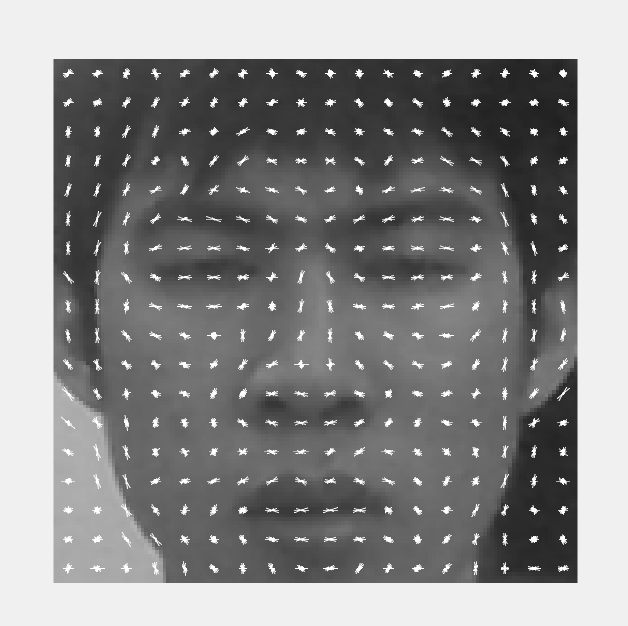
\includegraphics[scale=0.45]{HOG_extraction.png}
\caption{ Biến đổi HOG }
\label{fig:ts}
\end{figure}

\subsection{Phát hiện và khoanh vùng vị trí khuôn mặt (Face Detection)}
\begin{itemize}
    \item Trước hết, phải nhận biết được là khuôn mặt nằm ở đâu trong khung hình. Nhóm sử dụng \textbf{thuật toán Viola-Jones} được Paul Viola và Michael Jones trình bày vào năm 2001. 
    \item Thuật toán Viola-Jones có khả năng phát hiện vật thể nhanh (có thể dùng trong real-time)
    \item Có 4 giai đoạn:
    \subitem - Haar Feature Selection
    \subitem - Creating an Integral Image
    \subitem - Adaboost Training
    \subitem - Cascading Classifiers
\end{itemize}
\subsubsection{Haar Feature Selection}
\begin{itemize}
    \item Khuôn mặt con người thường có những đặc điểm chung nh:ư độ sáng vùng pixel ở mắt thường nhỏ hơn ở trán, và ở mũi
    \item Do đó sự kết hợp các thuộc tính sau tạo nên những thuộc tính đặc trưng cho khuôn mặt con người:
    \subitem - Vị trí và kích thước: mắt, mũi, ... 
    \subitem - Giá trị: các gradient có hướng của độ lớn các pixel (hay sự khác biệt về độ sáng giữa vùng màu sáng và tối khi lướt qua 1 vùng cụ thể trong bức ảnh).
    \subitem - Giá trị này được tính bằng tổng độ lớn của các pixel trong vùng màu đen trừ đi tổng độ lớn của các pixel trong vùng màu trắng
    \item Có nhiều dạng của Haar feature khác nhau ( Hình \ref{fig:haar} )
    \item Đối với 1 bức ảnh cụ thể, ta có nhiều thuộc tính được phân biệt bởi (vị trí, độ scale, loại). Ước tính có gần 160,000 thuộc tính
    
    
\end{itemize}

\begin{figure} [H]
\centering
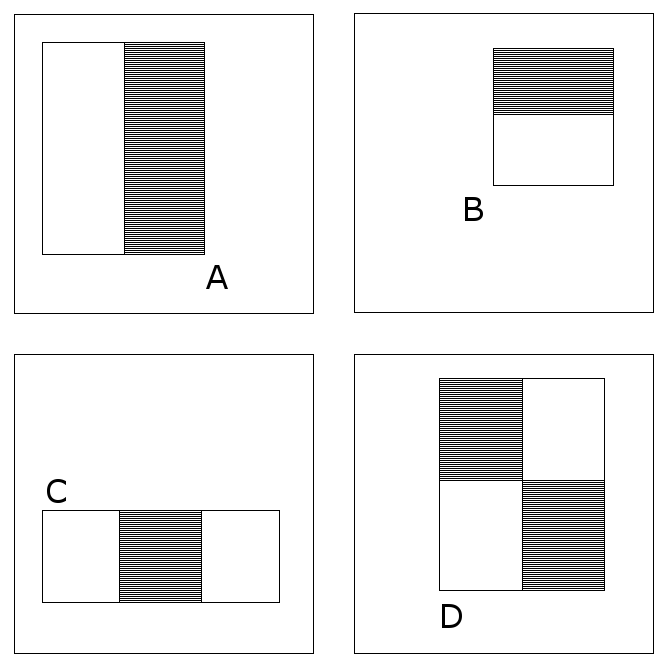
\includegraphics[scale=0.45]{haar.png}
\caption{ Haar feature}
\label{fig:haar}
\end{figure}

\subsubsection{Tạo bức ảnh "tích phân"}
\begin{itemize}
    \item Đối với việc tính toán tổng của 1 vùng các pixel với kích thước khác nhau, vị trí khác nhau. Điều này dẫn đến việc tính toán có độ phức tạp cao.
    \item Để có thể tính toán được các thuộc tính Haar, ta sẽ dùng bức ảnh "tích phân" 
    \item Trong bức ảnh "tích phân", giá trị tại 1 điểm pixel sẽ là tổng của vùng pixel nằm trong hình chữ nhật giới hạn bởi điểm gốc và điểm pixel đó 
\end{itemize}

\begin{figure} [H]
    \centering
    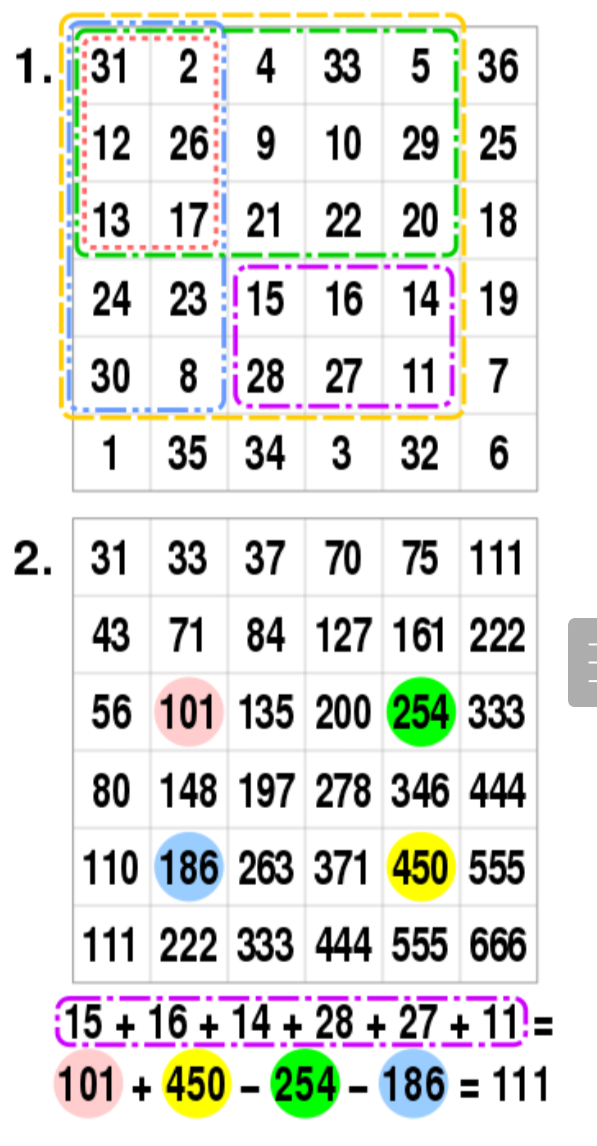
\includegraphics[scale=0.45]{integral_image.png}
    \caption{ Integral Image }
    \label{fig:integral_image}
\end{figure}

\subsubsection{Adaboost Training}
\begin{itemize}
    \item Là một thuật toán của học máy
    \item Mục đích là tìm ra những thuộc tính tốt nhất trong 160,000+ thuộc tính 
\end{itemize}

\begin{figure} [H]
    \centering
    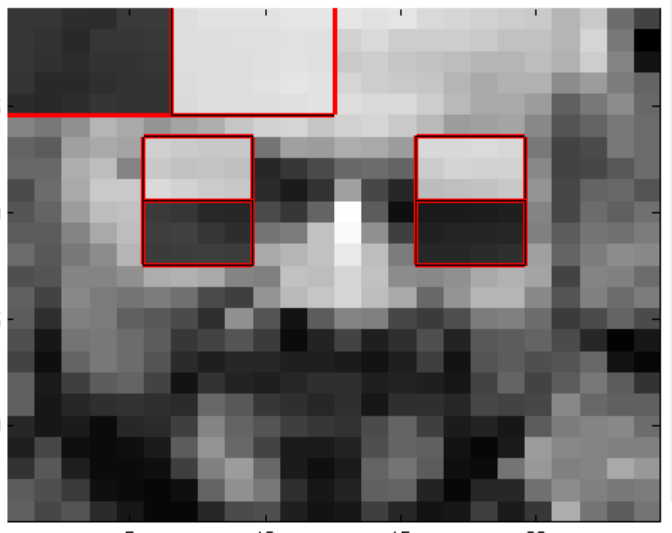
\includegraphics[scale=0.45]{adaboost.png}
    \caption{ Adaboost training  }
    \label{fig:adaboost}
\end{figure}

\subsubsection{Cascading Classifier}
\begin{itemize}
    \item Thay vì lướt toàn bộ trong bức ảnh với nhiều kích cỡ khác nhau để tìm xem đó có phải là khuôn mặt hay không, chúng ta có thể cải thiện bằng cách loại bỏ đi những vùng mà được cho là không có khuôn mặt người trong đó, chỉ tập trung vào những vùng có khả năng có khuôn mặt người  
\end{itemize}

\subsection{Nhận diện danh tính người (Face Recognition)}
\begin{itemize}
    \item Dựa vào dữ liệu đã train và dự đoán khuôn mặt đó là của người nào và độ tin cậy là bao nhiêu \% 
\end{itemize}

\begin{figure} [H]
    \centering
    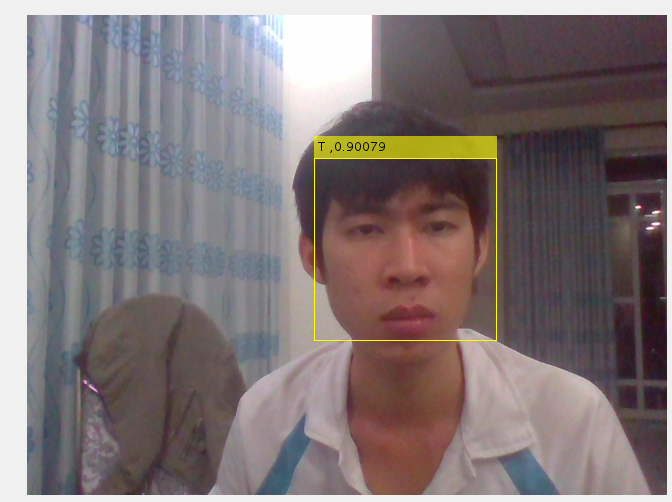
\includegraphics[scale=0.45]{face_recognition.png}
    \caption{ Face Recognition }
    \label{fig:ts}
\end{figure}

\section{Kết quả thu được}

\section{Kết luận}
\subsection{Điểm mạnh}
\begin{itemize}
    \item Có thể nhận diện khuôn mặt trong thời gian thực
\end{itemize}

\subsection{Điểm yếu}
\begin{itemize}
    \item Thời gian train có thể lâu nếu dữ liệu lớn
    \item Kết quả sẽ không chính xác nếu người đó thay đổi kiểu tóc, cạo râu hay để râu
\end{itemize}





\section{Tài liệu tham khảo}
\begin{itemize}
    \item  Viola, Jones: Robust Real-time Object Detection, IJCV 2001
    \item Torbert, Shane (2016). Applied Computer Science (2nd ed.). Springer
\end{itemize}
%%%%%%%%%%%%%%%%%%%%%%%%
%%%%%%%%%%%%%%%%%%%%%%%%%%%%%%%%%


 
\end{document}

